\chapter{System Design \& Implementation}\label{C:work_done}

One characteristic of this project is that it focuses on a recommendation system for a mobile application, rather than a website application. This affects how users will interact with the system, since with a mobile interface, the small form factor influences design decisions such as what ratings should be collected from users. Since existing components of WOTM are done in the programming language Ruby, it means we are confined to this language. In addition, the data in the application has already been modelled, including the food dishes, restaurants, and users. The only data not modelled is the data required for the recommender system such as the user ratings and food preferences etc.   

\section{Design Decisions}

For designing a recommendation system, the user goals and user experience has to be considered. This section details the design decisions regarding the recommendation process and the consideration how it influences the user experience in WOTM.

\subsection{Open source projects}

Open source projects can be utilised to fit the projects specific needs, as opposed to the alternative of starting from scratch. This saves time, allowing the focus to be on the CF techniques themselves. The open source community has a range of available projects. In particular, a range of machine learning libraries are available that incorporate various types of CF techniques. Spotify \cite{annoy} have an open-source project called Annoy \cite{annoy} that uses a CF neighbourhood approach. Recommendable \cite{recommendable} also uses a CF neighbourhood approach and is written in Ruby, making it easy to integrate with existing WOTM components. There were many other open-source projects such as EasyRec \cite{easyrec}, Apache Mahout \cite{mahoutaction}, Lenskit \cite{lenskit} among others, containing a range of CF techniques. 

Investigations on these systems led to the discovery of PredictionIO, the main open-source project used in this project.

\subsubsection{PredictionIO}

PredictionIO is an open-source machine learning server that supports multiple algorithms, and supports rapid build and deployment of predictive applications \cite{predictionio, predictionio2}.

\begin{figure}
\centering
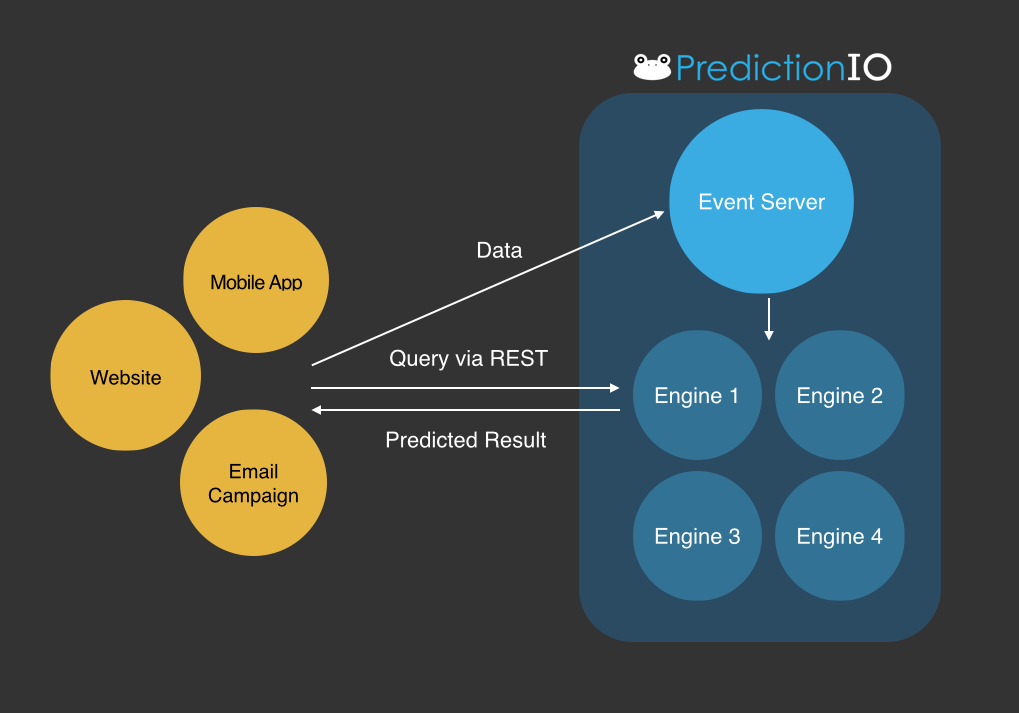
\includegraphics[scale=0.35]{images/predictionIO}
\caption{ How external applications interact with PredictionIO \cite{predictionio}. In this case, WOTM can interact with PredictionIO through REST queries which enable communication and data between the two applications.}
\label{fig:predictionIO}
\end{figure}

Figure \ref{fig:predictionIO} represents how PredictionIO is made to integrate with existing applications \cite{predictionio}. Data such as rating events from WOTM is sent to the Event Server where it is stored on PredictionIO. PredictionIO uses a distributed database that is easily scalable. Data from the event server is then used by algorithms from the engines to learn recommendations. These engines are deployed as distributed web services. WOTM can query these deployed engines to retrieve the top N recommendations for a specific user. 

The main advantage of using PredictionIO is that engines can be easily swapped out making it easy to examine and evaluate various CF techniques. This saves time, switching the main focus on CF algorithms rather than configuring settings to accommodate various technology and tools.

Additionally, these engines implement a DASE architecture \cite{predictionio}. DASE stands for Data, Algorithms, Serving, and Evaluator. These components are considered to be independent in the engine which allows for separation of concerns. Implementation of various algorithms can be applied at the Algorithms stage, and enables results from the various algorithms to be combined at the Serving stage to produce hybrid CF approaches for recommendations.

PredictionIO already contains a range of customizable engines, including engines that use Alternating Least Squares (Section \ref{als}) for CF. The PredictionIO community is active and new engines are frequently being produced. Additionally, there is concise documentation and support available. For these reasons, we found PredictionIO to be our best candidate and decided to use it. 

\subsection{User Experience}

A mobile application encourages user interaction that differs from that of a website. For instance, users are encouraged to use touch events to navigate through pages or to perform certain actions. This leads to design decisions that accommodate such interactions, making it easier for users to perform tasks on mobile applications. The user experience affects the collection of ratings from users, in turn, affecting the frequency in which users will rate food dishes. This will influence the quality of recommendations. Additionally, if the recommendation process is slow, users are less likely to continue using the application. On the other hand, if prediction accuracy is not accurate, then users will be recommended items that may not be of interest. Trade-offs must be considered.  

\subsection{Explicit Feedback}

Recommender systems rely on different types of input data \cite{koren2009matrix}. Explicit data is referred to as a direct record of someones interest of an item. For example, Netflix collects star ratings for movies, and TiVo users collect data from having a thumbs up or thumbs down directly indicating that they like or dislike a particular item \cite{koren2009matrix}. These events are mapped directly in the ratings matrix, and explain directly how a user feels about an item. 

\subsubsection{Binary Ratings vs Ternary Ratings vs Likert Scale Ratings}

Although prediction-accuracy is important, it is not the only factor that a recommender should focus on, and acts as one facet in wide range of facets \cite{martin2009recsys}. \citeauthor{martin2009recsys} \cite{martin2009recsys} explains that the goal of a recommender system is to improve user experience, however, designing a recommender system to fit a specific application remains a challenge, and recommender system ratings should be based on the user experience. By focusing on user experience, users will be able to easily rate food dishes, in turn, leading to the system collecting more information for the recommender system from ease of use. For this reason, a simple model allowing users to easily rate a dish such as a binary rating (Like/Dislike) or a ternary rating (Like/Neutral/Dislike) is preferred over Likert scale ratings. This provides simplicity, but means recommendations will not be as accurate as Likert scale ratings such as 1-5 stars or 1-10 stars. By easing the user experience for rating food dishes it can increase data collection at the expense of accuracy. \citeauthor{movieratings} \cite{schafer2007collaborative, movieratings} found users provided more ratings that had options to ``Like" or ``Dislike" than users with only one rating option. 

Using Likert scaled ratings mean that we learn more about the user preferences because of the scaled factor indicating how much the user likes a dish or not. This means that model based CF techniques are able to learn what the user likes and dislikes faster leading to more accurate recommendations. However, a Likert scale system such as a 1-5 star rating also has problems. For example, if a dish had a 5 star rating, it may mean only 1 or 2 people have rated the dish. Ratings such as 3.5 stars may mean that it is a good dish, but from the way it is displayed, may seem otherwise. By displaying what other users think of an item, the active user tends be influenced by the opinions of others, leading to bias ratings \cite{interface}. An example would be a user rating a dish higher than they would normally because the food dish has an average of 4.5 stars. This can lead to inaccurate recommendations for the active user in the long term, because users may be influenced by others opinion \cite{interface}. \citeauthor{interface} \cite{interface} argues that the way ratings are collected and displayed, influence how others will rate the dish. Therefore, considerations have to be taken into account to understand how the user will perceive and interact with the recommender system.  

A trade-off to consider is whether or not accurate recommendations are more important than the user experience. Since WOTM aims at being a mobile application, the limitations are the small form factor that mobile phone screens have. With a Likert scale rating system, the user has to be shown these possible options in order to rate a dish. This can take up additional space that is not available on small screens. Because of this, having a 1-5 star rating system may degrade the user experience as opposed to a simple like/dislike rating system. 

For a mobile application, the predicted score of the recommender system may not matter a great deal. For instance, a recommender system could predict two dishes the user may like based on previous rating patterns. The first dish is predicted with a 90\% predicted score, and the second dish is predicted with a 70\% predicted score that the user will like these dishes. But is the difference in prediction scores important if the user likes both dishes? As long as the recommender system has provided the user with dishes they like, the accuracy between those predicted dishes do not drastically matter. In addition, dishes with higher predicted scores may seem like obvious choices the user may have already tried, whereas dishes with a lower predicted score may lead to less obvious dishes that they may like, but have not tried yet. A recommender system using boolean or ternary values may eventually reach prediction accuracy similar to using likert scale ratings. Although this will happen in the long term, new ratings will most likely lead to less accurate predictions that join the system in the short term until more ratings are collected. 

Foursquare \cite{foursquare} is an application that asks users to rate items according to a series of questions. These questions consist of ``What do you like about this place?", ``What is this place known for?" and so on. From these questions they are able to infer a particular rating for the item, as well as collect data from users to give more accurate recommendations. This rating system may risk users not rating the items because of the long list of questions it asks. \cite{martin2009recsys} explains that part of the challenge is to design interfaces ``that give users control over the recommendation process without overwhelming the user or rendering the tool too complicated for novice users." 

For these reasons, we found that simple like/dislike events would best suit the collection of data for the recommender system because of the simplified structure which increases the user experience. The recommender system can be extended to take in additional events that may portray additional information such as a ``want" indicating that a user ``wants" a dish but has not yet tried it before. However, caution must be taken as more events will affect the user experience of the application, but may lead to more accurate recommendations. 

\subsection{Implicit Feedback}

When explicit feedback is not available, implicit data can be used to infer preferences from users \cite{koren2009matrix}. Implicit feedback is referred to as an indirect reflection of someones interest in an item. Implicit feedback can be from observing user behaviour. This could include click through data, browsing history, the way users react to certain events, search patterns, and so on \cite{koren2009matrix}. Implicit feedback can be collected to increase the accuracy of recommendations to users by being combined with explicit feedback, or can fill in the ratings matrix when explicit events are not available, alleviating the ``Cold Start" problem as it makes the matrix more dense. 

\subsubsection{Additional Events}

Netflix \cite{koren2009matrix} and other sites such as Amazon.com \cite{schafer2007collaborative} use implicit feedback such as views and purchase history in their recommender systems. These events indicate some form of interest in the user, however are less practical to apply for a mobile application. For example, on a website, many products are able to be shown to the user. When a user selects a product it will indicate some form of implicit feedback such as the user is interested in that product. With the WOTM mobile application, it can be difficult showing a range of food dishes to users because of the small screen size. This can make it difficult to collect additional implicit feedback. As well as this, purchase history and similar events are not practical because users are unlikely to indicate they have purchased a dish after they have tried it. Explicit ratings such as Like and Dislike already infer they have tried the dish, which make purchase history redundant. The implicit event of commenting on a dish may provide valuable information, perhaps commenting on a dish means that there is a strong interest or disinterest a user has about a specific dish. However, this is impractical because we do not know if the comment is good or bad without using extraction techniques.

A consideration is the collection of feedback based on how users feel about the recommendations produced by the system. This can be used to gather additional information, to make predictions more accurate. For instance, a user can indicate that they Liked/Disliked the recommendation that was shown to them, or they could skip it altogether meaning they do not have an opinion about it. The flaw in this method is that recommendations may be dishes the user has not tried yet. Therefore, they may keep skipping through recommendations and provide no valid feedback to them. Although this may happen, an assumption is that user ``Like" events may be used for a dish the user has not yet tried, but is interested in. For these reasons, implicit events are not used in our recommendation system.

\section{Default Recommendation Engine}

This section explains what has been implemented according to the design decisions in the previous section.

\subsection{E-Commerce Engine Template}

PredictionIO \cite{predictionio} provides many template engines, some of which use CF algorithms to make recommendations to users. In particular, there is a template engine that uses ALS to learn the latent factor vectors in SVD. This engine is called the ``E-Commerce Recommendation Engine", and will be built upon to suit the use case of ``Find Good Items" in this project. 

The E-Commerce Recommendation Engine \cite{predictonio} is written in the programming language Scala and is made to provide personalised recommendations for e-commerce applications. This engine uses Alternating Least Squares (ALS) which is learning algorithm to discover the latent factors in SVD. This means the model is built from training on users ratings, identifying patterns and learning about recommendations the users may be interested in. The training process occurs offline to minimize the computation cost for online use, providing fast recommendations. The engine comes with the following (out of the box) functionality \cite{predictionio}.
\begin{enumerate}
 \item Exclude out-of-stock items
 \item Provide recommendation to new users who sign up after the model is trained
 \item Recommend unseen items only (configurable)
 \item Recommend popular items if no information about the user is available
\end{enumerate}

Default events in the engine are \textit{view} events and \textit{purchase} events. In order to receive recommendations, the engine must be first built, trained, and deployed. Once the recommendation engine is deployed, queries can be sent to the engine by creating a client object, and specifying the user id, and the number of recommendations for a user as seen in Listing \ref{code:query_recs}.  

\begin{lstlisting}[caption={Query for recommendations}, label={code:query_recs}]
# Create client object to connect to the recommender system.
client = PredictionIO::EngineClient.new('http://localhost:8000')
# Query PredictionIO for 3 recommendations for user 1.
recommendations_list = client.send_query(user: 1, num: 3)
# puts recommendations_list
\end{lstlisting}

The list of $n$ recommendations from Listing \ref{code:query_recs} are shown in Listing \ref{code:recs}, outputting the recommended items for user 1 in JSON format containing the item id, and the predicted preference score for each item. 
\begin{lstlisting}[caption={Recommendations for user 1}, label={code:recs}]
{
  "itemScores":[
    {"item":"4","score":0.82},
    {"item":"12","score":0.74},
    {"item":"5","score":0.43}
  ]
}
\end{lstlisting}

By default, the engine recommends \textit{popular} items to new users based the highest \textit{viewed} items. The advantage of this is that new users get to see recommendations immediately, however the disadvantage is that it may create bias results in the engine because popular items will only be seen by new users. This means new users will only rate the \textit{viewed} items, causing problems in the recommender engine. 

Another feature is the handling of unavailable items. Queries can be sent to the recommendation engine to indicate the item is no longer available. This seems applicable in WOTM if food vendors decide that they are no longer selling a particular food dish, then these items can be disregarded in the recommendations. 

\section{Implementation} \label{implementation}

Modification of the default recommendation engine was performed to take into account binary ratings: ``Like" and ``Dislike", removing the \textit{view} and \textit{purchase} events. The CF algorithm is modified in the engine to consider a ``Like" event as positive result, giving it a preference value of 1.0. In contrast, the algorithm was modified in the engine to consider a ``Dislike" event to be a negative result, giving it a preference value of -1.0. Since users may change their minds about liking or disliking a food dish, the CF algorithm is modified to only consider the most recent Like/Dislike ratings from the user. Filtering in this recommendation system has also been added based on users preferences such as their meat type, their cuisine type, and their food type. This makes it possible for recommendations to be given to users with strict food preferences such as vegetarian users, filtering any food dishes containing meat. As well as this, users can see recommendations that are within their price range, if specified. This allows users to receive food dish recommendations that they can afford.

\subsection{Popularity Function} \label{subsection:popularity}

The default recommendation engine originally provides a popularity function that recommends the highest count of \textit{view} ratings on each item. For binary ratings, this popularity function is insufficient to provide popular recommendations since it does not take into binary ratings such as Likes and Dislikes. Therefore, the popularity function in the default recommendation is overridden by a new popularity function implementation based on binary ratings ``Likes/Dislikes". 

In cases of the ``Cold Start" problem, where a new user has joined the system but has not rated any items, recommendations based on popular food dishes are a way of recommending items that have a higher chance the user will like the food dish compared with random recommendations. There are many factors considered when using a popularity function based on binary events (Likes/Dislikes). An example of this, would be the case where a food dish has a high number of likes, but also a high number of dislikes. For a problem such as this, a simple equation that takes the average would suffice such as the equation: $average= likes/(likes+dislikes)$ \cite{popularity}. However, the average does not work if an item has few ratings. For example, a food dish with only 1 ``Like" rating would be ranked at the top of the recommendations list since it has a 100\% positive ratio. However, this should not be the case, since the amount of users having rated the item is small in comparison with other food dishes \cite{popularity}. 

The Wilson Score Confidence Interval \cite{wilson1927probable, popularity} is a statistical equation that can be applied in the context of popularity, considering binary ratings (Like/Dislike). The lower bound of the Wilson Score Confidence Interval has been applied for sorting popular comments in Reddit \cite{reddit}, and also has been applied in Yelp \cite{yelp_pop}.

The lower bound of the Wilson Score Confidence Interval is defined in equation \ref{wilson}  \cite{wilson1927probable, popularity}. The $\hat{p}$ is the observed fraction of ``Like" ratings on the item, $n$ is the number of total binary ratings (Like/Dislike), $z$ is the confidence interval, and $z_{\alpha/2}$ is the $(1-\alpha/2)$ quantile of the standard normal distribution \cite{popularity}.    

\begin{equation} \label{wilson}
\left(\hat{p} + \frac{z^2_{\alpha/2}}{2n} - z_{\alpha/2} \sqrt{[\hat{p}(1-\hat{p}) + z^2_{\alpha/2}/4n]/n}\right)/(1 + z^2_{\alpha/2}/n)
\end{equation}

The lower bound of the Wilson Score Confidence Interval estimates the portion of ``Like" ratings with respect to uncertainty from having a small number of rating samples \cite{popularity}. Given the number of ratings, a confidence interval is used to estimate the real portion of positive ratings within the confidence interval \cite{popularity}. Therefore, an implementation of Wilson's Score Confidence Interval is used at a 95\% confidence interval to recommend popular items to the user in the situation where there is insufficient ratings to provide personalised recommendations. 
Popular items can be recommended based on this function by providing an extra parameter to the query shown in Listing \ref{code:popular}. This returns $n$ recommendations sorted by the Wilson Score Interval, returning preference scores between 0.0 and 1.0.

\begin{lstlisting}[caption={Query for popular recommendations}, label={code:popular}]
# Query PredictionIO for popular recommendations.
recommendations_list = client.send_query(user: 1, num: 3, popular: true)
\end{lstlisting}

\subsection{Recommender System Implementations} \label{algorithms}

Fine-grained rating information such as 1-5 star ratings contain fine-grained preferences from users which may be beneficial for the recommender system. Binary ratings lack this fine-grained information, therefore, the recommender system should utilise binary ratings to best influence the recommendations. For example, using multiple explicit ratings such as Likes and Dislikes could provide worse recommendations than using 1-5 star ratings produced by the ALS algorithm since 1-5 star ratings provide more information. To understand how binary ratings affect the recommender system, implementation of various ALS algorithms are explored to utilise the information in binary ratings.

\subsection{Baseline Popularity Predictor System} \label{baseline}

The baseline predictor provides a base performance which is used to compare the performance of CF algorithms against. In the experiment, a baseline predictor provides non-personalised recommendations, recommending food dishes to users based on the popularity of food dishes. The popularity of a food dish is based on the ``Like" ratings and ``Dislike" ratings from users. The popularity function used in the recommender system is the Wilson Score Confidence Interval described in Section \ref{subsection:popularity}. The recommender system outputs a list of top $n$ recommended food dishes, each containing a score based on the popularity of the food dish. Since the Wilson Score Confidence Interval normalises the popularity score between ranges of 0.0 to 1.0, an optimal threshold is applied which determines food dishes that will be recommended. The optimal threshold is found from a Receiving Operating Characteristic (ROC) curve in Sections \ref{roc}, \ref{auc}).

\subsection{Single SVD System}

\begin{figure}
\centering
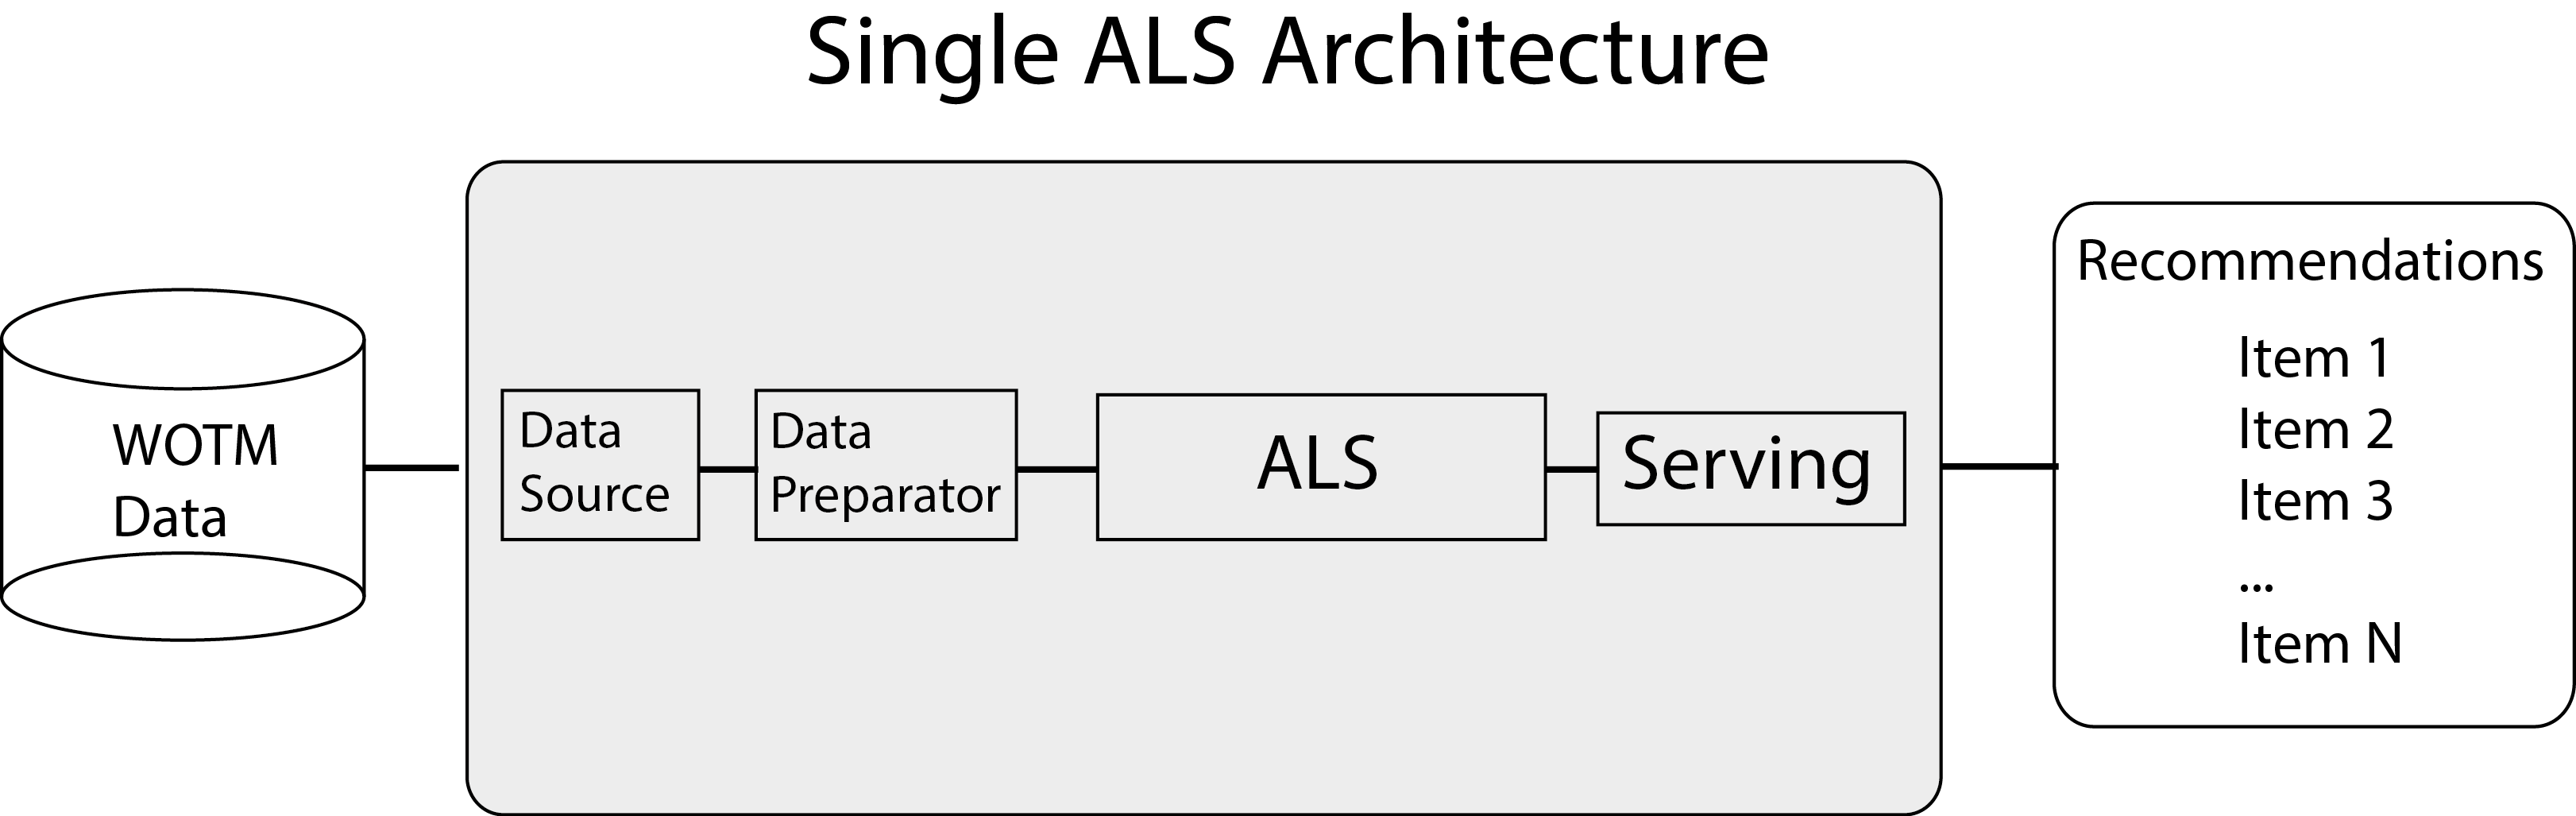
\includegraphics[scale=0.5]{recent_images/Single_ALS_architecture.png}
\caption{Single SVD Architecture where the model uses binary ratings (Like/Dislike) in the same model.}
\label{fig:single_architecture}
\end{figure}

The Single SVD algorithm uses the model described in Section \ref{implementation}. The architecture of the system can be seen in Figure \ref{fig:single_architecture}. Data from WOTM is sent to the Data Source. Data contained within the Data Source can be selected to be sent to the Data Preparator where data prepossessing can occur. After this stage, the data is passed to the SVD algorithm, where all the results are processed in the Serving layer. Post-processing can occur in the Serving layer for purposes such as combining results from different algorithms. The Serving layer then provides recommendations to the user.

The Single SVD contains both rating events of Like and Dislike in the model. Since SVD works by capturing latent factors from user and item vectors, having the binary ratings of Like and Dislike in the same model may not accurately represent the correlation between Like and Dislike ratings from users. The recommendations may be skewed towards one rating event. For example, if there are more users that have disliked a specific item compared to the number of likes, the feature vector captured by that item may result to negative values in the feature space. This may lead to inaccurate recommendations, where having another rating such as ``Dislikes" actually deviates away from the main goal and can cause noisy information in the algorithm. For this reason, a more practical approach would be to separate each rating event into an independent SVD algorithm, and then combine the results from both algorithms at the end of the Serving phase. 

\subsection{Dual SVD System} 

\begin{figure}
\centering
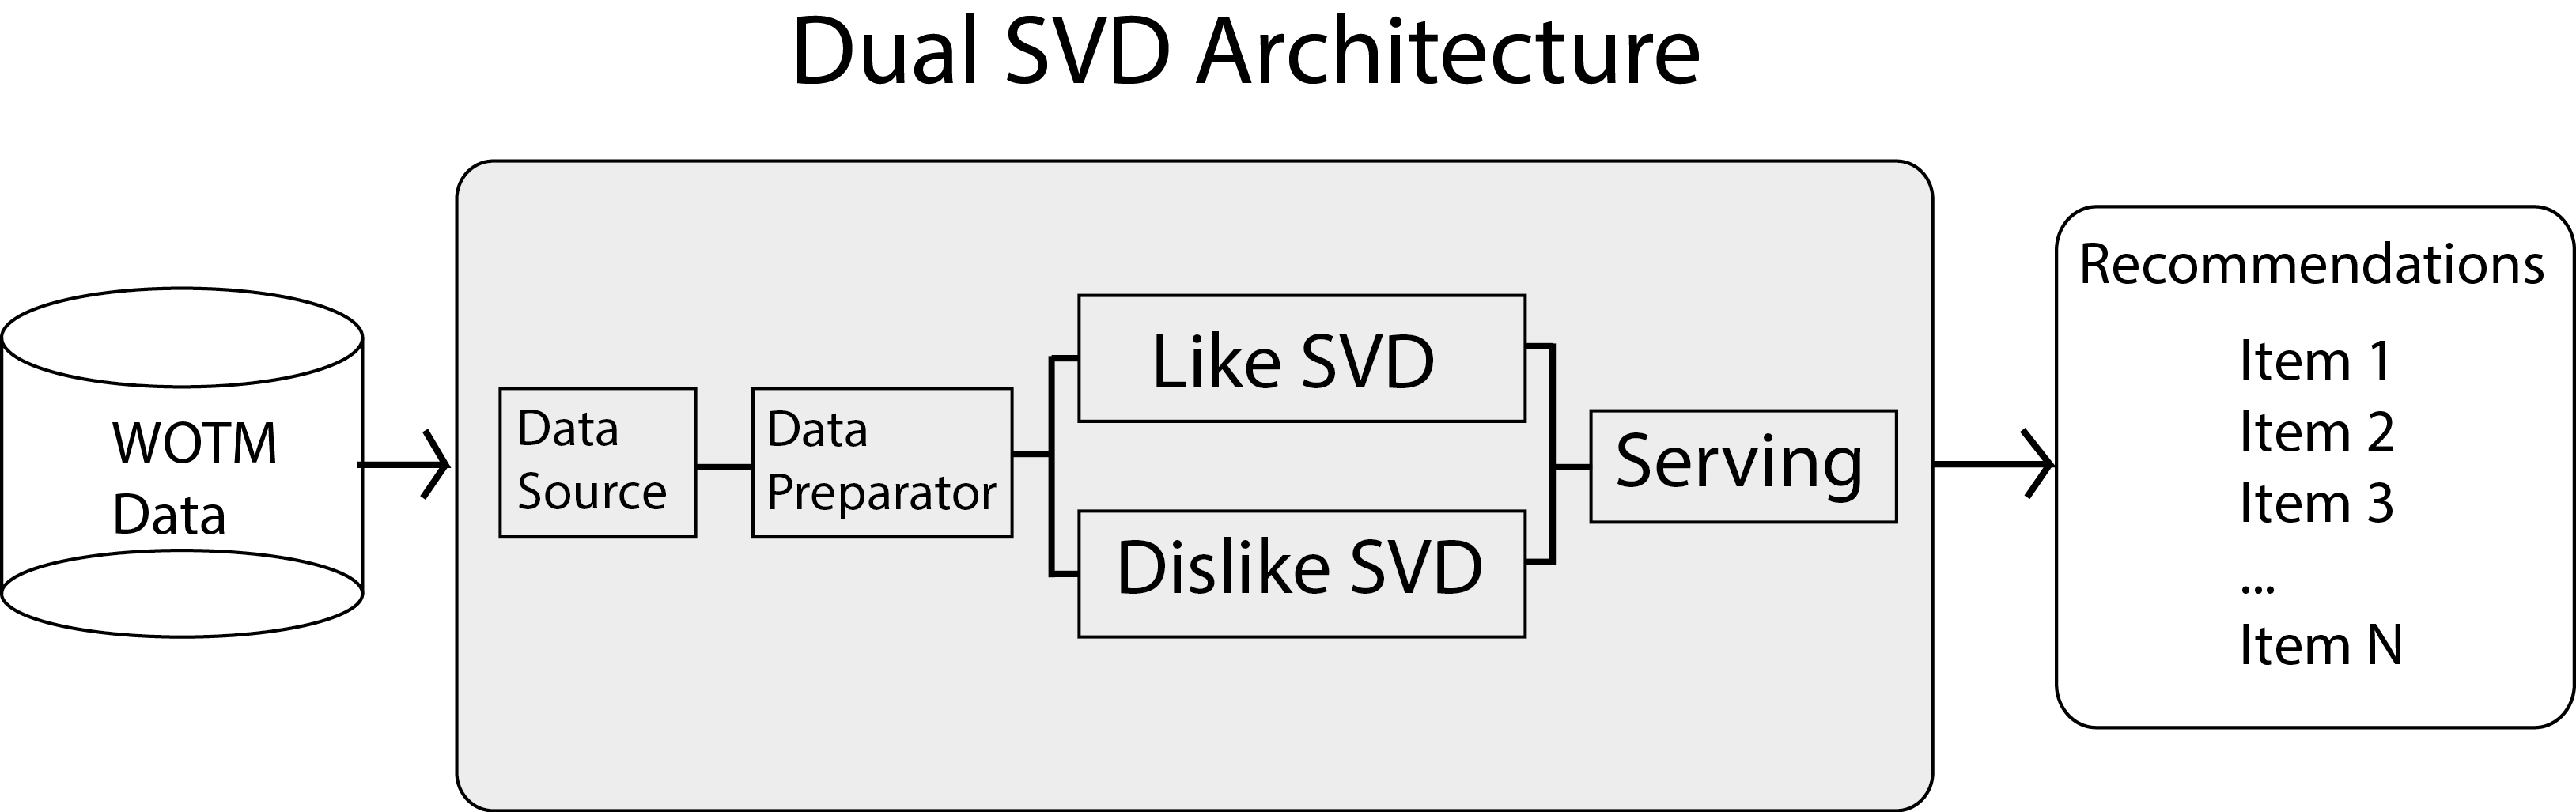
\includegraphics[scale=0.5]{recent_images/Dual_ALS_architecture.png}
\caption{Dual SVD Architecture where binary ratings are separated into a different model, and the results are merged in the Serving layer to provide correlated recommendations.}
\label{fig:dual_architecture}
\end{figure}

This model differs from the Single SVD as it separates the ``Like" ratings from the ``Dislike" ratings and stores each type of rating in separate models. It then merges the results to try and find a correlation between the binary ratings of Like/Dislike from users, resulting in the final recommendation list. The Dual SVD architecture can be seen in Figure \ref{fig:dual_architecture}.

Rating events are given preference values where both ``Like" and ``Dislike" ratings correspond to a positive value of 1.0. By separating the events into two separate models, one model is able to predict the most ``Liked" food dishes, while the other model is able to predict the most ``Disliked" food dishes. Since both ratings of ``Like" and ``Dislike" are represented b a positive preference value, recommendations from each model will return the highest positive item scores. Therefore, merging these scores at the Serving phase where the ``Disliked" item scores are subtracted from the ``Liked" item scores. This should provide strongly correlated recommendations based on both ratings since the final recommendation list will contain food dishes where the predicted ``Disliked" food items have been negated from the recommendations list. This provides accurate recommendations since the relationship between both events are taken into consideration.

Since the ratings have been separated into different models, the ratings are now considered implicit ratings due to SVD not knowing explicitly what each rating is. A Weighted-Alternating Least Squares (W-ALS) \cite{implicit, abergerrecommender} is used to learn the latent vector factors for implicit ratings, shown in Equation \ref{eq:3}. 

% A binary preference value of 1 indicates that the user likes the item, and a binary preference of 0 indicates no preference for the user. Additionally, implicit events also have a confidence value associated with it. These confidence values represent the confidence levels of the binary preference values being true. In this case, preference values for the \textit{view} and \textit{purchase} events correlate to the value of 1. Multiple identical events such as a user viewing the same item multiple times correlate to higher confidence levels since the confidence level is an aggregation of preference values. This means that there is a higher confidence level that the binary preference value is true, in this case, that the user will like the item because the user viewed or purchased the same item multiple times, recommendations taking this into account \todo{how? how can this be calculated?}. 

\begin{equation}\label{eq:3}
\displaystyle min_{q*,p*} \sum_{ (u,i) \in K} c_{ui}(b_{ui} - q_{i}^T p_{u})^2 + \lambda (\| q_{i} \|^2 + \| p_{u} \|^2 )
\end{equation}

In this equation, \begin{math} c_{ui} \end{math} is the confidence level that can be tuned during cross validation, and \begin{math} b_{ui} \end{math} is the binary preference value. 

\subsection{Hybrid SVD System}

\begin{figure}
\centering
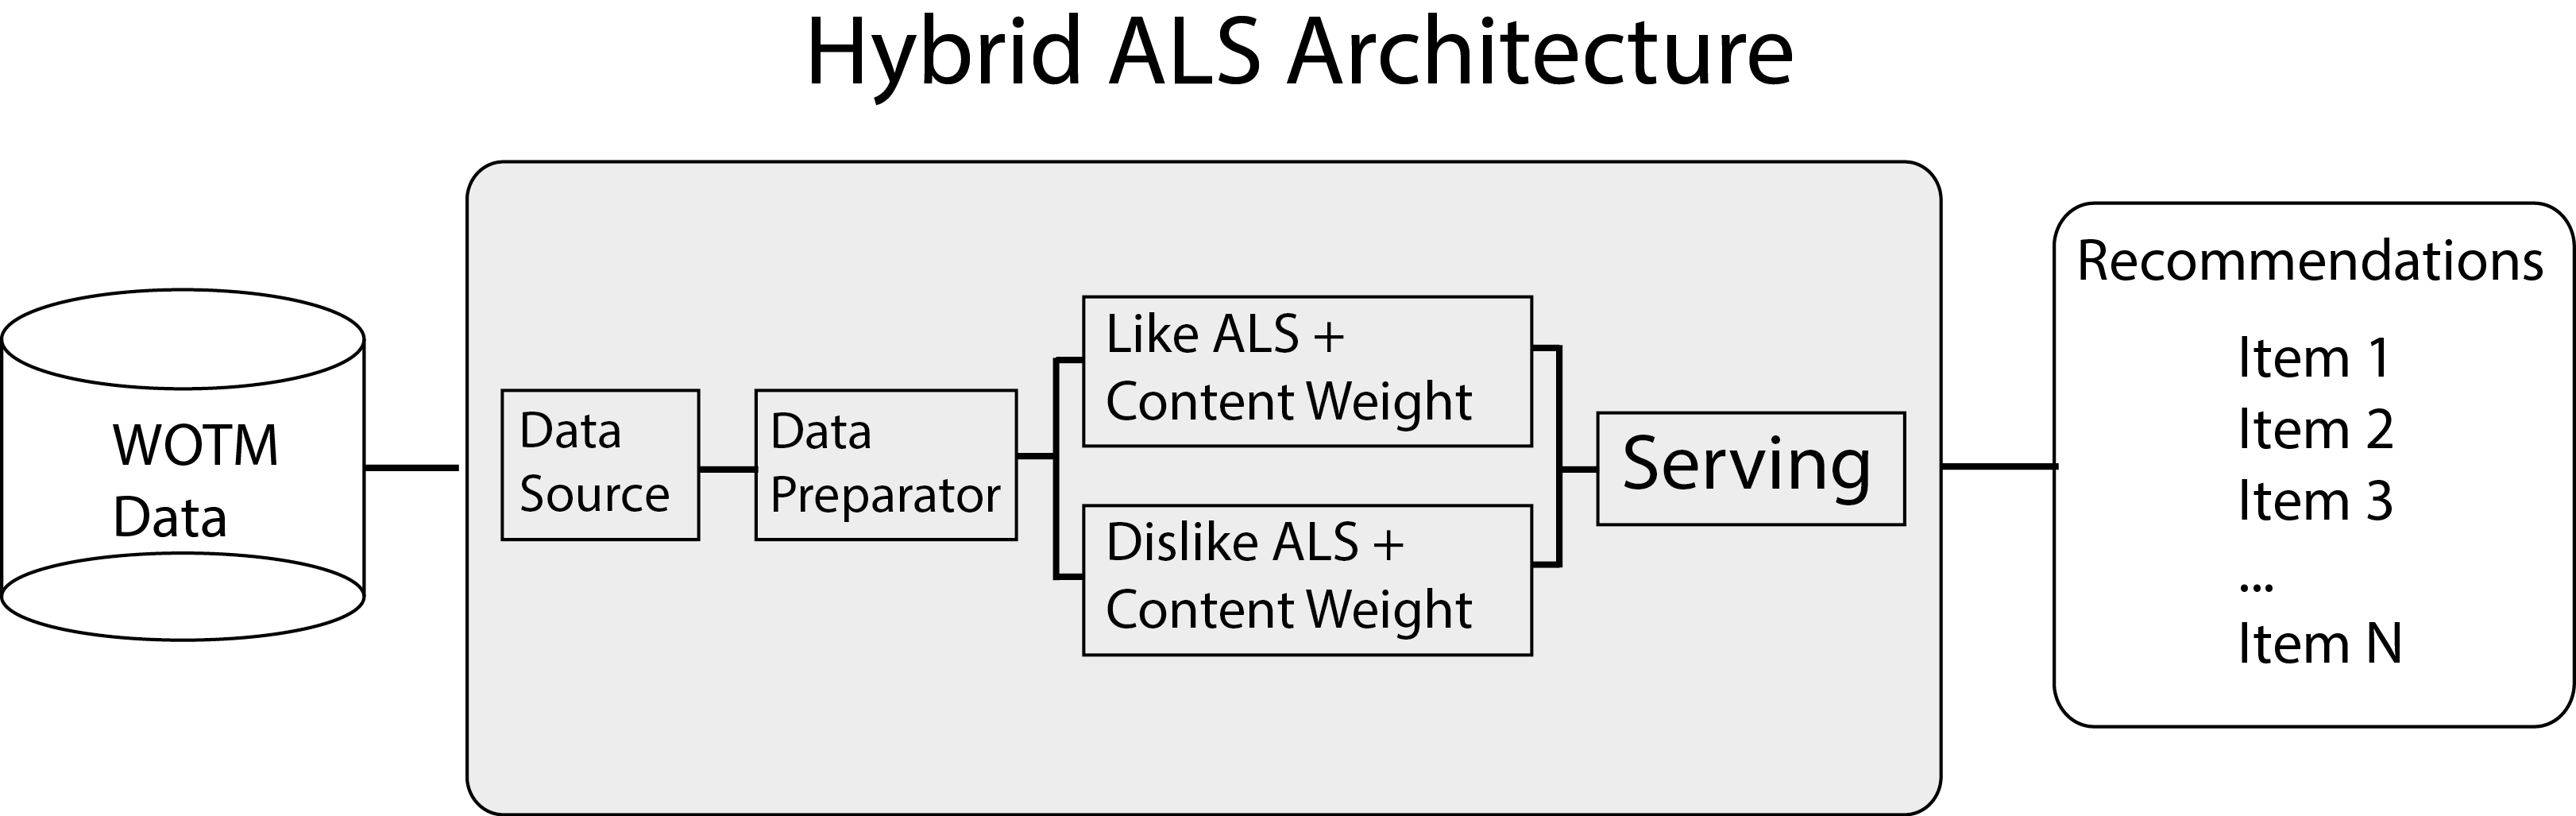
\includegraphics[scale=0.5]{recent_images/Hybrid_ALS_architecture.png}
\caption{Hybrid SVD Architecture where binary ratings are separated into a different models where content is boosted from users food preference. Results are merged in the Serving layer to provide correlated and content-boosted recommendations.}
\label{fig:hybrid_architecture}
\end{figure}

The Hybrid SVD System uses a Weighted \cite{spiegel2010hybrid} and a Switching \cite{spiegel2010hybrid} hybrid CF approach. The Hybrid SVD System is an extension of the Dual SVD System but includes boosting the score of recommendations based on attributes that the user prefers. 

The architecture of the Hybrid SVD System is shown in Figure \ref{fig:hybrid_architecture}. Similar to the Dual SVD System, it uses two models to provide correlated recommendations to users based on binary ratings (Like/Dislike). In each of these models, the content preference of the user is boosted based on how the user feels about the content. A value is determined representing the strength of the boost. This value should be determined through empirical studies. Results from both models are linearly combined before recommendations are shown to users. 

Food dishes contain attributes that make up the food dish. For example, a food dish may contain ingredients, a food type, a meat type, and a cuisine type. At a high-level, food dishes may be associated with a restaurant, a type of category, or a type of location where the food dish can be purchased. Since WOTM is currently in development, only broad granularity of food dishes have been specified: food type, meat type, and cuisine type. This meta data is sent to the recommendation engine along with the food dishes. Therefore, recommendations can be only boosted based on these attributes. 

When a user has not yet rated any food dishes but has specified food attribute preferences such as preferred food type, meat type or cuisine type, then recommendations based on this content can be given to users. This is a Switching \cite{spiegel2010hybrid} approach that is invoked when there is insufficient information for CF to be performed. This has been designed to work when the model is online, rather than learning these content preferences offline. This is because attribute preferences can help mitigate the ``Cold Start" problem for new users. For example, new users that log into the WOTM mobile app can be asked to indicate food preferences before they start rating food dishes. Immediate recommendations can be based on these food preferences from the users. These recommendations are provided by specifying extra parameters to the query as seen in Listing \ref{code:query_hybrid}. The weighting of the content can be configured since parameters have been included in the recommendation system, called ``preferenceWeight". Figure \ref{code:hybrid_recs} demonstrates the recommendations returned from the Hybrid CF system.

\begin{lstlisting}[caption={Query for recommendations based on hybrid CF}, label={code:query_hybrid}]
# Query PredictionIO for 2 recommendations based on a hybrid approach.
recommendation = client.send_query(user: 9, positivePreferences: ["Chicken"], negativePreferences: ["Pie", "Salad"], num: 2)
\end{lstlisting}

\begin{lstlisting}[caption={two recommendations for user 9 based on hybrid CF}, label={code:hybrid_recs}]
{
  "itemScores": [
    {
      "name": "Fried Chicken",
      "item": "231",
      "score": 1.1902140651574058,
      "contents": [ "fried chicken", "chicken", "meat" ]
    },
    {
      "name": "Wedges",
      "item": "280",
      "score": 1.1308979710816303,
      "contents": [ "cafe", "potato" ]
    }
}
\end{lstlisting}

\subsection{Item SVD System}

The Item SVD System performs an item-based CF technique based on previously liked food dishes from users. It uses the same architecture as the Dual SVD System in Figure \ref{fig:dual_architecture}. It differs from Dual SVD as it performs item-based CF by using the cosine similarity measure to find similar items based on the factors in the item vectors. Item-based filtering is performed when an extra query parameter is specified and sent to the recommendation engine. The specified query takes in an array of item ids the current user has previously liked as shown in Listing \ref{code:query_items}. Implementation of the item parameter in the query was done to provide real-time recommendations.

\begin{lstlisting}[caption={Query for recommendations based on Item-based CF}, label={code:query_items}]
# Query PredictionIO for 10 recommendations based on item-based CF for user 1
recommendations = client.send_query(user: 1, items: [1,2], num: 10)
\end{lstlisting}

The cosine-similarity measure is used to find similar items, returning a list of items based on the cosine angle, where a cosine angle of 1 between two items represents the highest similarity, and a cosine angle of -1 between two items represents the opposite. Recommendations are provided to users based on items with the highest similarity scores. 